\pdfbookmark[0]{Mainbody}{title}
\pagestyle{fancy}
\newgeometry{left=3cm, right=3cm, top=2.79cm, bottom=2cm}
\fancyhead[R]{\textsf{CPT106: User's manual for Car Parking System}}
\fancyhead[L]{}
\fancyfoot[C]{Page \thepage \ of \pageref{LastPage}}
\renewcommand{\headrulewidth}{2pt}
\renewcommand{\baselinestretch}{1.5}
\setcounter{page}{2} 
%\linespread{1.5}
{\rmfamily\selectfont
\vspace{-1ex}

\hypertarget{project-develop}{%
\section{Project Develop}\label{project-develop}}

\hypertarget{develop-analyze-and-plan}{%
\subsection{Develop Analyze and Plan}\label{develop-analyze-and-plan}}

The development plan is a crucial component for the successful
completion of our C++ project. It outlines the project\textquotesingle s
overall objectives, timeline, and division of work. The following is our
group\textquotesingle s development plan for developing this project.

\begin{enumerate}
\def\labelenumi{\arabic{enumi}.}
\item
  Define project objectives:

  Prior to commencing the project, we will establish clear objectives
  and requirements. First, we had a quick discussion to determine the
  topic (Group C: parking system). After that, we divided into two
  groups: development group and documentation group. At the same time,
  we decided to use WeChat for intra-group communication and Git for
  code and document progress synchronization. The development and
  documentation teams choose their own toolchains and internal
  divisions. Finally, the team leader creates the GitHub repository and
  sets up the main-dev-feature development stream.
\item
  Division of Work:

  We will assign specific responsibilities to each team member based on
  their strengths, skills, and interests. As a team, we will
  collaboratively determine the tasks and deliverables for each phase of
  the project. This will promote effective teamwork and ensure that each
  team member contributes to the project\textquotesingle s success.

  a. Development Team:

  Two team members will be responsible for the actual development of the
  C++ project. The development team members communicated quickly,
  designed a project solution with high cohesion and low coupling (see
  below), and quickly implemented it. It is worth mentioning that one of
  the project team members, whose computers are all based on the GNU
  Linux operating system, will complete the project using platform - and
  compiler-independent syntax.

  b. Documentation Team:

  The other two team members will be responsible for preparing the
  project report and documentation. They will collect and organize
  relevant information about the project, including the design
  decisions, implementation details, and test results. They will ensure
  that the project report is well-structured, concise, and accurately
  represents the work completed. In addition, because Git is based on
  version control of changes to text files, it does not work well with
  MS Word files (such as .docx). The documentation team uses \LaTeX
  to write documents, a format that uses plain text to record the
  original content and can easily generate pdf files.
\end{enumerate}

By following this development plan, we aim to successfully complete the
C++ project within the given timeframe while meeting all the project
requirements and delivering a high-quality solution.

\hypertarget{project-architecture}{%
\subsection{Project Architecture}\label{project-architecture}}

In order to balance development efficiency and code quality, the team
adopted a frontend-backend separation architecture design.
Frontend-backend separation, also known as UI and code logic separation,
has several benefits. Firstly, it allows for a clear separation of
concerns, enabling frontend developers to focus on designing an
intuitive and visually appealing user interface (UI), while backend
developers can concentrate on implementing complex business logic and
data processing. This division of labor promotes specialization,
enhances productivity, and enables parallel development. Secondly, it
facilitates scalability and flexibility by providing the ability to
upgrade or replace either the frontend or backend independently, without
affecting the other component. Lastly, it promotes code reusability and
maintainability, as changes made to one component are less likely to
impact the other, simplifying debugging and reducing the overall
development and maintenance effort.

\begin{center}
  \centering
  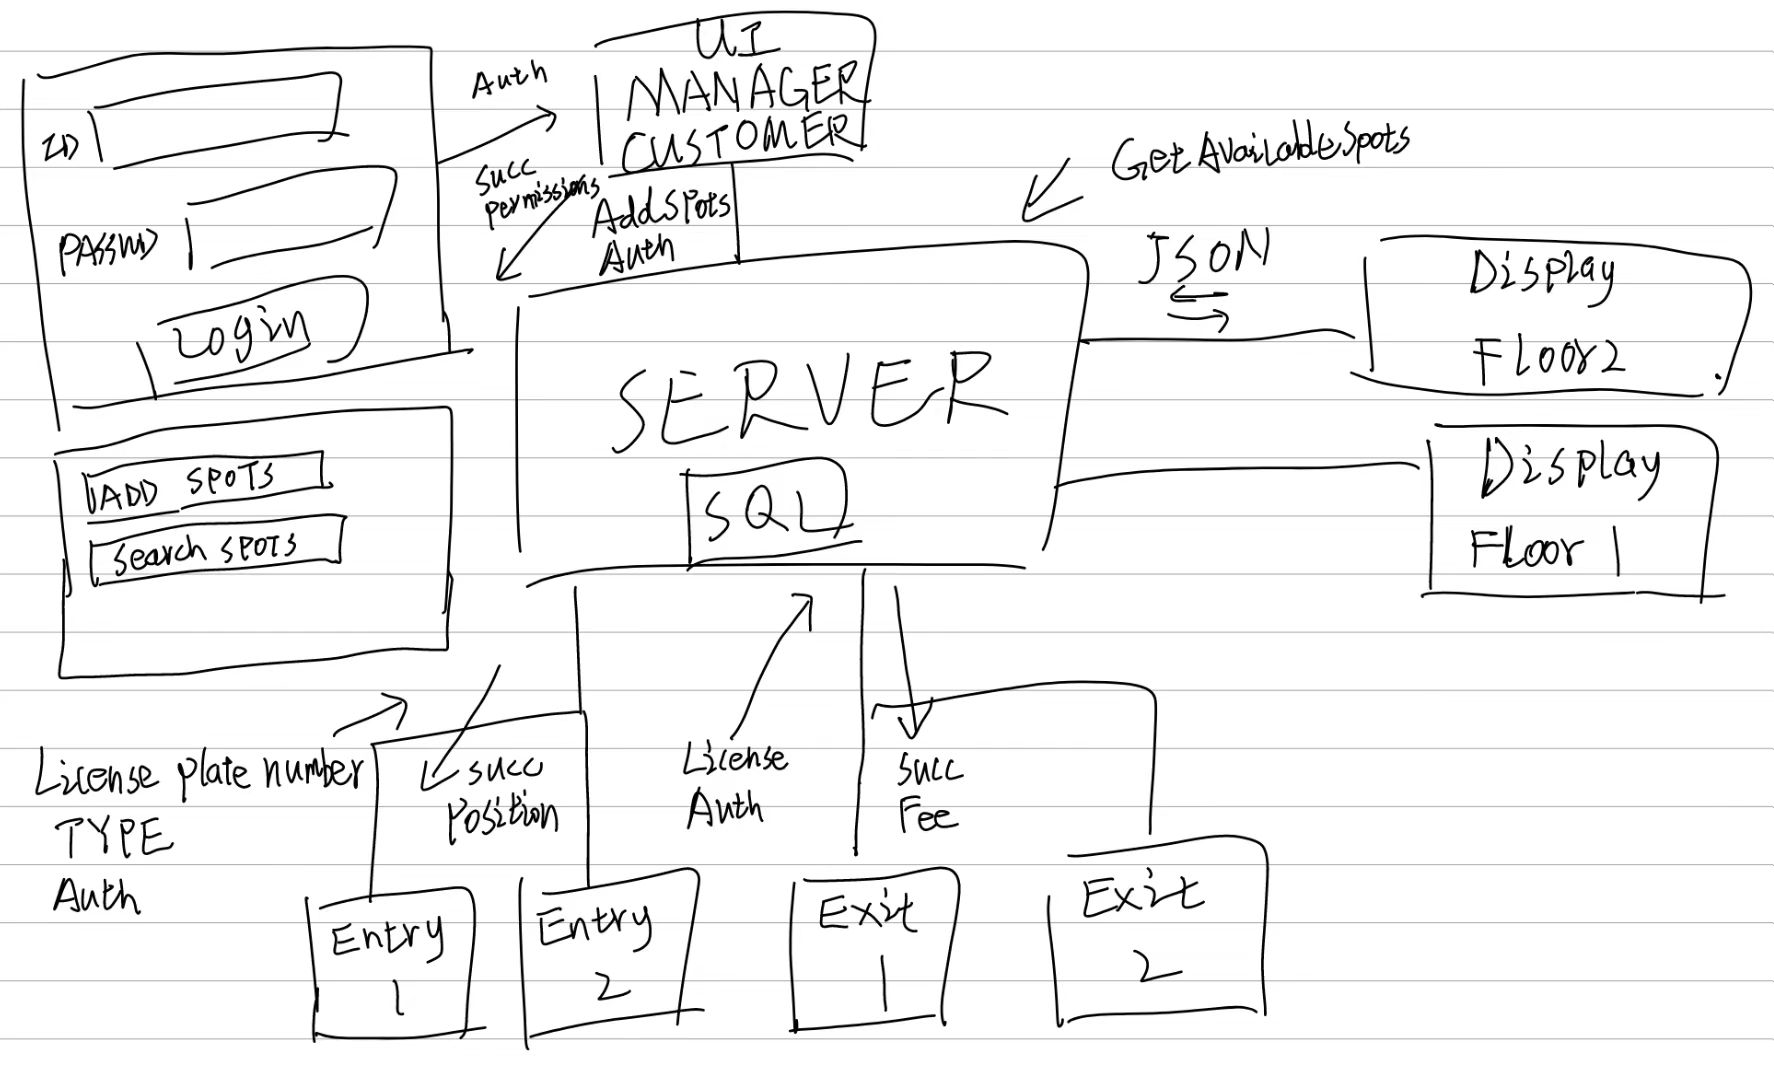
\includegraphics[width=0.8\textwidth]{D:/OneDrive/School/CPT106/Group Project/GM/2023_CPT106_Group/report/project_developing/1.png}
  \captionof{figure}{Project Architecture}
\end{center}


The frontend of our project utilizes the Qt framework, a popular
cross-platform application development framework. Qt provides a
comprehensive set of tools and libraries for building graphical user
interfaces (GUIs) efficiently. We leverage the Qt Designer tool to
visually design the UI components, arrange layouts, and define their
properties. Additionally, the Qt User Interface Compiler (uic) tool
converts the UI design files into C++ code that can be seamlessly
integrated with the backend logic. By leveraging the Qt toolchain, we
can streamline the frontend development process, enhance code
reusability, and achieve a consistent and visually appealing user
interface across different platforms.

\begin{center}
  \centering
  \includegraphics[width=0.8\textwidth]{D:/OneDrive/School/CPT106/Group Project/GM/2023_CPT106_Group/report/project_developing/2.png}
  \captionof{figure}{Running on linux.}
\end{center}

\begin{center}
  \centering
  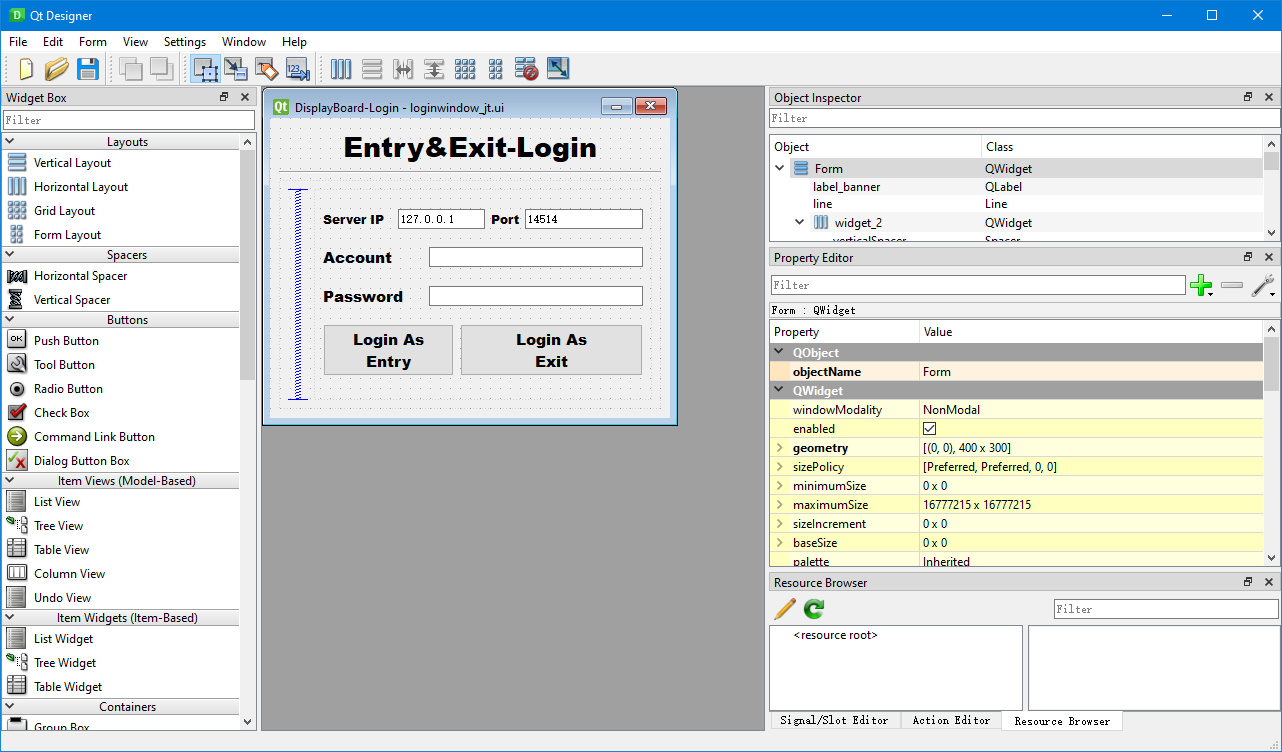
\includegraphics[width=0.8\textwidth]{D:/OneDrive/School/CPT106/Group Project/GM/2023_CPT106_Group/report/project_developing/3.png}
  \captionof{figure}{Designer Page}
\end{center}

The communication between the frontend and backend of our project is
facilitated using the TCP (Transmission Control Protocol) protocol. TCP
provides a reliable and connection-oriented communication channel
between the client (frontend) and server (backend). This ensures that
data packets are delivered in order and without loss or corruption.

To facilitate the exchange of data between the frontend and backend, we
utilize the JSON (JavaScript Object Notation) format for serialization
and transmission. JSON is a lightweight and widely supported data
interchange format that allows for easy representation and parsing of
structured data. By using JSON, we can effectively serialize complex
data structures into a human-readable format that can be transmitted
over the TCP connection, enabling seamless communication and data
exchange between the frontend and backend components of our project.

\begin{center}
  \centering
  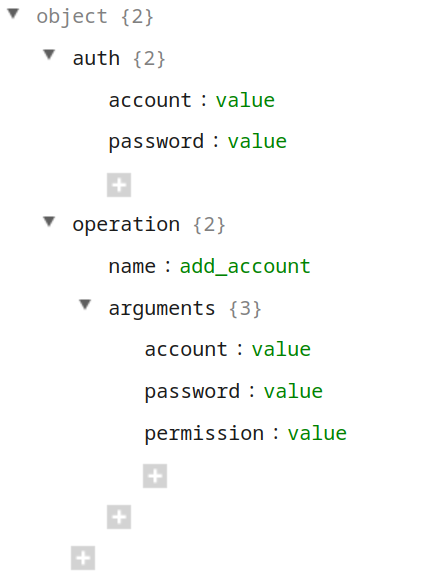
\includegraphics[width=0.7\textwidth]{D:/OneDrive/School/CPT106/Group Project/GM/2023_CPT106_Group/report/project_developing/4.png}
  \captionof{figure}{JSON Data Example}
\end{center}

\hypertarget{develop-test}{%
\subsection{Develop Test}\label{develop-test}}

Testing is a crucial step in the development process. At the end of the
testing, the code is delivered to the customer. It ensures that the
software functions as intended, identifies any defects or issues, and
verifies that the system meets the specified requirements. In the case
of a frontend-backend separated project, testing becomes essential to
ensure the seamless interaction between the UI and backend components.
The testing process for our project involves separate unit testing for
both the UI and the backend components, followed by integration testing
to ensure their seamless interaction.

We first tested each modular unit independently to ensure that the
layout, appearance and behaviour of the front-end UI elements matched
the design, and that the back-end units performed the expected actions
and produced the expected output correctly.

After all the UI annd backend components have undergone thorough unit
testing, integration testing takes place. It verifies that the frontend
and backend functionalities work together harmoniously, ensuring proper
data exchange and preserving the desired system behavior.

After testing, we merge the code from the dev branch to the main branch,
indicating that the code has been accepted and moved from development to
maintenance status.
}
